\documentclass{article}
\usepackage[utf8]{inputenc}
\usepackage{graphicx}
\usepackage{amsmath}
\usepackage{amsfonts}
\usepackage{hyperref}
\usepackage{color}

\setlength{\parindent}{0em}
\setlength{\parskip}{0.5em}

\title{Bird embedding}
\author{Li-Ping Liu}
\date{}


%%%%%%%%%%%%%%%%%%%%%%%%%%%%%%%%%%%%%%%%%%%%%%%%%%%%%%%%%%%%%%%%%%%%%%%%%%%%%%%%%%%%%%%%%%
% some notations
\newcommand{\wt}{\boldsymbol{\rho}}
\newcommand{\obswt}{\boldsymbol{\beta}}
\newcommand{\emb}{\boldsymbol{\alpha}}

%%%%%%%%%%%%%%%%%%%%%%%%%%%%%%%%%%%%%%%%%%%%%%%%%%%%%%%%%%%%%%%%%%%%%%%%%%%%%%%%%%%%%%%%%%
\begin{document}

\maketitle

\section{Introduction}

The eBird data consists of checklists of bird observations. The figure below shows some sites having checklist submissions on Manhattan island. eBird project even includes a \href{http://ebird.org/ebird/livesubs}{\textcolor{blue}{webpage}} that shows real-time submissions. 


\begin{figure}[h]
    \centering
    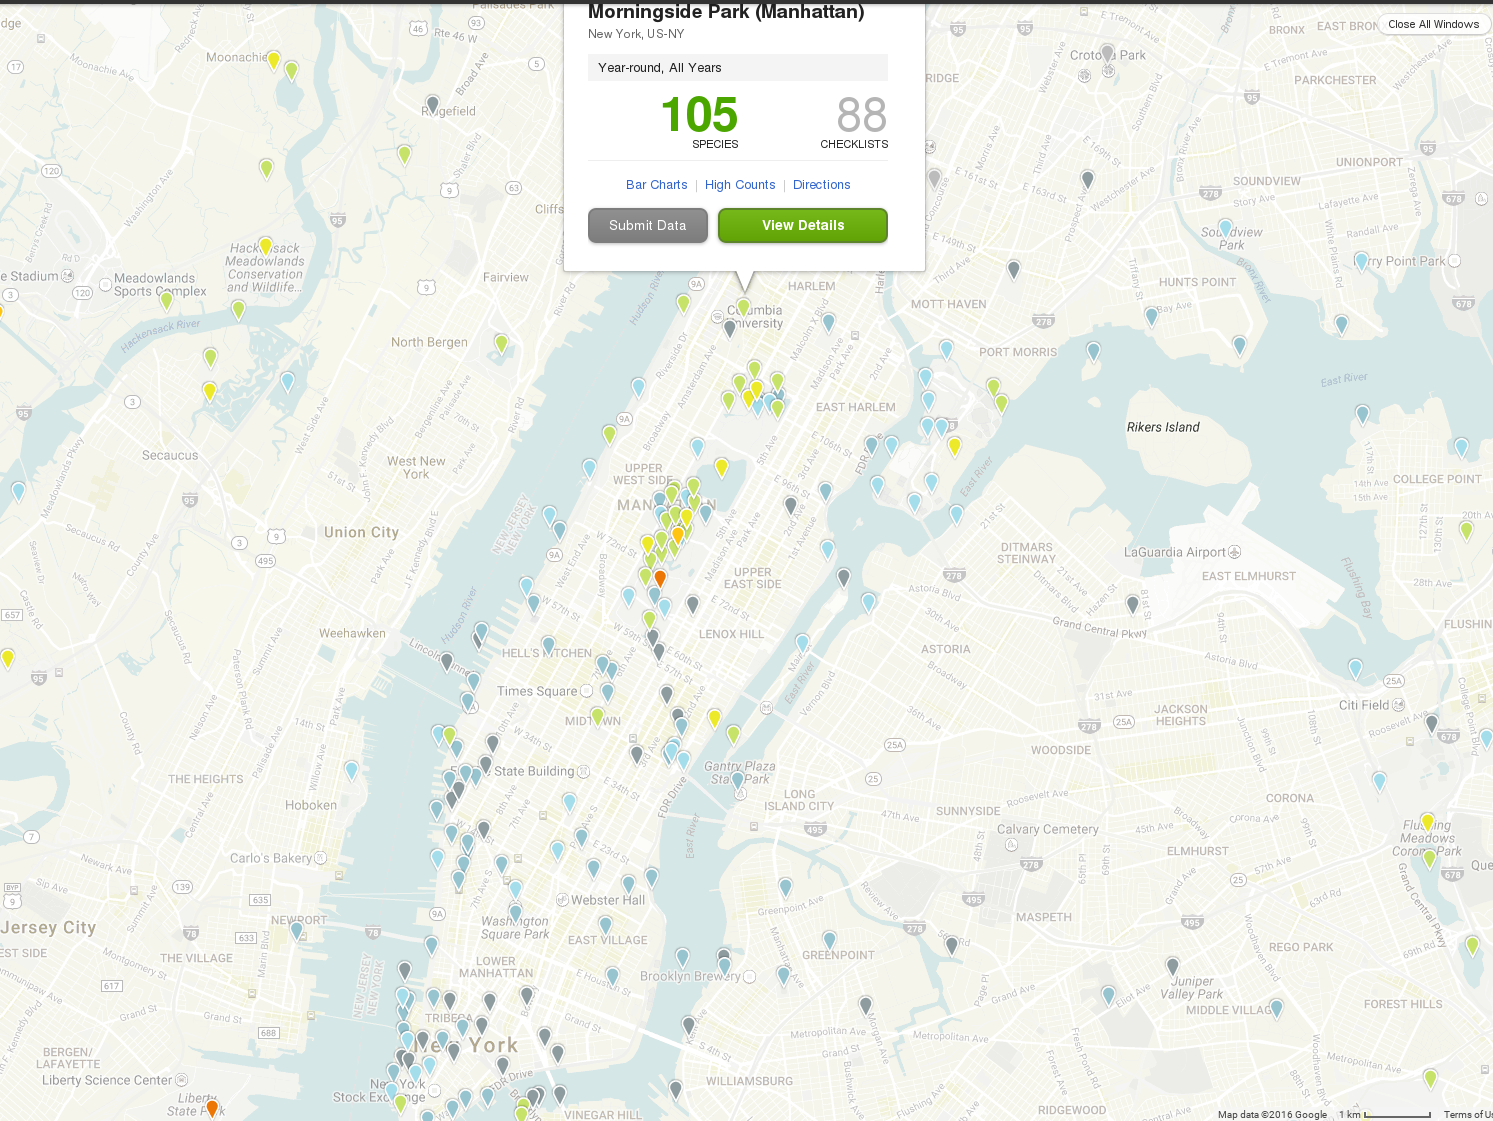
\includegraphics[width=0.8\textwidth]{figures/ebird-checklist-manhattan.png}
    \caption{eBird checklist submissions on Manhattan island. (I believe) Checklists are aggregated by a number of sites for better plot. The location at CU is mistakenly labeled as Morningside Park. Zoom in for better view. }
    \label{fig1}
\end{figure}


Each checklist contains its location (latitude \& longitude), time point, and a list of bird counts for 953 species. Two sets of covariates are associated to each checklist. The first set ($\approx$ 12) of covariates describe the environmental information, such as elevation, temperature, and vegetation coverage, and explain why the bird is there. The second set ($\approx$4) of covariates are about the observation process and states how the observation is made, such as the type of observation (staitionary, traveling, area survey, etc.) and duration of observation. 

There are about 6 million checklists during the last 5 years (from 2010 to 2014). 

In this work, we would like to discover bird relations by bird embedding. The idea of bird embedding originates from word embedding in NLP, where various relations among words are discovered[citation of word embedding]. We project that applying the embedding technique to the bird data will give some interesting results. 

Dispite its similarity with word embedding, there are new problems to consider for bird embedding. 
\begin{itemize}
\item Large quantity of data, which has 6 millions observations.
\item Rich information about checklists. In another word, checklists are not from the same distribution. We should construct a model in which environmental covariates expain presence/absence of species, and bird embedding captures interactions among species.  
\item Locations near each other should have similar distribution of birds, not only because they share similar covariates, but also because birds fly around. How to smooth the distribution?
\item How can we explain the embedding result? Making recommendation may not be a good idea here. 
\end{itemize}


\section{Bird Embedding}

The first model to consider is the combination of exponential family embedding and the exposure model.

In the embedding model, we essentially need to define the conditional distribution of the bird count of a species in a checklist given its {\it context}. Since we are interested in relationships among bird species, the {\it context} of a bird count is the vector of bird counts of other species in the same checklist. In view of the generality of context, we can define the context of a bird count flexibly, for example, as bird counts of other species averaged over checklists within some radius of the current observation. The average may give more stable results, but we will consider this later. 

The exposure model can be used to describe the observation process. Mathematically, it plays the role of down-weighting zero entries in the observation matrix. In another word, a species is not observed either because no such bird lives there or because it is not detected by that observation. If the model choose the second explanation, then model makes little effort to fit the zero value. We will see this after we have defined the model formally.  

Let's define the model. Suppose there are $N$ checklists, and let $i$, $1 \le i \le N$, index checklists. In the data there are $J$ species, each of which is indexed by $j$, $1 \le j \le J$. In each checklist $i$, $y_{ij}$ birds are observed for species $j$. 

For each checklist, the feature vector $\mathbf{x}_{i}$ brings some information of the observation process. The probability $u_{ij}$ of observing each species $j$ is calculated as $u_{ij} = \mathrm{logistic}(\obswt_j^\top \mathbf{x}_i + \beta^0_j)$, where $\obswt_j$ is a parameter, and $\beta^0_j$ is the bias term. The indicator $b_{ij}$ of observing species $j$ at checklist $i$ is sampled from Bernoulli distribution with probability $u_{ij}$. 
\begin{eqnarray}
b_{ij} &\sim& \mathrm{Bernoulli}(u_{ij}).
\end{eqnarray}

The observed count $y_{ij}$ is from Poisson distribution with rate $b_{ij}\lambda_{ij}$. 
\begin{eqnarray}
y_{ij} &\sim& \mathrm{Poisson}(b_{ij} \lambda_{ij}),
\end{eqnarray}
If $y_{ij} = 0$, the indicator $b_{ij}$ indicates whether the zero value comes from a poor dection or absence of the bird.
The underlying rate $\lambda_{ij}$ is calculated from the embedding. 

To define the embedding, we first define the {\it context} of $y_{ij}$, which consists of species with positive observations. 
\begin{eqnarray}
C_{ij} = \{j': y_{ij'} > 0, j' \neq j\}
\end{eqnarray}

The rate $\lambda_{ij}$ is defined in the embedded space, where each species $j$ is mapped to a vector $\emb_j$ and associate with another
vector $\wt_j$. 
\begin{eqnarray}
\lambda_{ij} &=& f\left(\wt_{j}^\top \sum_{j' \in C_{ij}} r(y_{ij'}) \emb_{j'} + \lambda^0_{j} \right) \label{lambda_exp} 
\end{eqnarray}
The function $r(\cdot)$ is used to scale large counts to a small range to avoid the domination of a large count in the summation. 
The function $f(\cdot)$ maps the value from $\mathbb{R}$ to $\mathbb{R}^{+}$ to get a valid rate for Poisson distribution. It can 
be defined as the exponential function or the softplus function ($f(x) = \log(1 + \exp(x))$). Different with traditional embedding, 
we also include an intercept term $\lambda^0_{j}$ as the base rate for each species.

The parameters $\alpha_j$, $\rho_j$, and $\beta_j$ are regularized by Gaussian priors. 
\begin{eqnarray}
\emb_j &\sim& \mathrm{Normal}(\mathbf{0}, \sigma^2_1 I), \\
\wt_j &\sim& \mathrm{Normal}(\mathbf{0}, \sigma^2_2 I), \\
\obswt_j &\sim& \mathrm{Normal}(\mathbf{0}, \sigma^2_3 I),
\end{eqnarray}
where $\sigma_1^2$, $\sigma_2^2$, and $\sigma_3^2$ are hyper-parameters, $\mathbf{0}$ represents a zero vector with proper length $N$, and $I$ represents the identity matrix of with proper size. 

The parameter $\wt$ and and $\emb$ explains the correlation among bird species. The correlation comes from either shared environmental factors or birds' interactions. If the embedding is to capture more about birds' interactions, the base rate $\lambda^0_{j}$ needs to explain more about environmental factors by including environmental covariates. 

\section{Inference}

In this section, we develop a varitional inference method to infer parameters of the model. 

\subsection{ E-step: calculating the posterior distribution of the indicator variable}

The posterior distribution $p(b_{ij} | y_{ij}, \lambda_{ij}, u_{ij})$ of the hidden indicator $b_{ij}$ is a 
Bernoulli distribution, and we denote its parameter as $q_{ij}$.
\begin{eqnarray}
q_{ij} = p(b_{ij} = 1 | y_{ij}, \lambda_{ij}, u_{ij}) = \left\{ \begin{array}{ll} 
1 & \mbox{if } y_{ij} > 0\\
\frac{u_{ij}\exp(-\lambda_{ij})}{1 - u_{ij} + u_{ij}\exp(-\lambda_{ij})} & \mbox{if } y_{ij} = 0
\end{array}
\right. \label{estep_q}
\end{eqnarray}


\subsection{M-step: maximizing the log-likelihood with respect to model parameters}

In the M-step, we want to maximize the following objective.
\begin{eqnarray}
LL(\wt, \emb, \obswt) &=& \sum_{ij} E_{b_{ij}} \Big[\log p\left(y_{ij} | b_{ij} \lambda_{ij} \right) + \log p\left(b_{ij} | \obswt_j^\top \mathbf{x}_{ij}\right)\Big] \nonumber\\
&=& \sum_{ij}  - (1 - q_{ij}) \log (1 +  \exp(\obswt_j^\top \mathbf{x}_i)) \mathbb{I}[y_{ij}=0] \nonumber \\
&& \hspace{0.5cm} + q_{ij} \Big( y_{ij}\log(\lambda_{ij}) - \lambda_{ij} - \log \big(1 + \exp( - \obswt_j^\top \mathbf{x}_i) \big) \Big) 
\end{eqnarray}
This equation shows how $q$ can downweight Poisson likelihood of zero counts. Since $q_{ij}$ equals to 1 when $y_{ij} > 0$
and is often less than 1 when $y_{ij} = 0$, Poison likelihood of non-zero counts averagely weigh more than that of zero counts. 

Take derivatives with respect to the parameters. 
\begin{eqnarray}
\nabla_{\wt_j} LL &=& \sum_{i}  q_{ij}^1 \left( y_{ij}/\lambda_{ij} - 1 \right)
\nabla_{\wt_j} \lambda_{ij} \label{grad_rho}\\
\nabla_{\emb_j} LL &=& \sum_{i}\sum_{j' \in C_{ij}}  q_{ij'}^1 \left( y_{ij'}/\lambda_{ij'} - 1 \right)
\nabla_{\emb_j} \lambda_{ij'} \label{grad_alpha}\\
\nabla_{\obswt_j} LL  &=& \sum_{i} - q_{ij}^0 \mathrm{logistic}(\obswt_j^\top \mathbf{x}_{ij}) \mathbf{x}_{ij} + q_{ij}^1 (1 - \mathrm{logistic}(\obswt_j^\top \mathbf{x}_{ij})) \mathbf{x}_{ij} \label{grad_beta}
\end{eqnarray}

With the softplus function, 
\begin{eqnarray}
\nabla_{\wt_j} \lambda_{ij} &=& \frac{\exp(h_{ij})}{1 + \exp(h_{ij})} \sum_{j' \in C_{ij}} r(y_{ij'}) \emb_{j'}, \\
\nabla_{\emb_{j}} \lambda_{ij'} &=& \frac{\exp(h_{ij'})}{1 + \exp(h_{ij'})}  r(y_{ij}) \wt_{j'},
\end{eqnarray}
where $h_{ij} = f^{-1}(\lambda_{ij})$.



\subsection{Maximization with Stochastic Gradient}

Combining the E-step with the M-step by appying $q$ values from (\ref{estep_q}) to the gradient calculations gives the gradient of 
the log-likelihood with respect to model parameters. Instead of calculating the exact gradient with all training instances, we 
only calculate a noisy gradient by using only one instance randomly drawn from the training set. Then we use AdaGrad to 
update model parameters with noisy graidents. Practically, the algorithm converges within 100,000 iterations. 

\subsection{Model Settings}

The model is defined to be flexible and can be configured in different ways.  
\begin{itemize}

\item[]{\bf downweighting zeros}: In the E step, $q_{ij}$ has the effect of downweighting zeros. We can also manually set $q_{ij}$ be a value 
in $[0, 1]$ to downweight zeros. (1) If we let the model fit $q$ values, we can either feed observation covariates into the model or not. 
In the latter case, the model will fit probability of indicators $b$ with the bias term only and then calculate $q$ accordingly.
(2) If we manually set $q$, we remove all likelihood terms related to the indicator and keep only Poisson likelihood. 
\item[]{\bf scaling context}: The counts exhibit large varince, and counts of some species are much larger than those of others. 
Therefore, in the context, the embedding will dominated by species with large counts, and large counts may also give extreme 
values of the Poisson rate $\lambda_{ij}$. One method is to divide each context count by the 95\% quantile of the counts of 
that species (scaling by column). The other method is to divide each count by the sun of counts in the context (scaling by row). 

\item[]{\bf intercept term:} Set $\lambda^0_{j} = 0$, or let the model fit $\lambda^0_{j}$.

\item[]{\bf link function:} $f(x) = \exp(x)$, or $f(x) = \log(1 + \exp(x))$.
\end{itemize}



\section{Experiment}

In the experiment, a subset of checklists are taken from a rectangular area that mostly overlps with Pennsylvania and the period from 
day 180 to day 210 in 2014. The subset has overall 5488 checklists (trips) and 181 bird species (items) with some species with fewer than 
5 checklists removed. Counts of each species are checked. Some anomalous counts with extrodinarily large numbers are set to the mean 
of counts of the species. The dataset is randomly split into two thirds as the training set and one third as the test set. The model is 
trained on the training set and tested on the test set for ten times on 10 different random splits. In each training run, the model 
is optimized on nine tenth of the training set and validated on the rest one tenth. For each random split, the negative predictive 
log-likelihood is recorded. 

The experiment starts the basic embedding model and sets $K = 10, \sigma_1 = \sigma_2 = \sigma_3 = 100, \lambda^0_j = 0, 
f(\cdot) = \exp(\cdot)$. The exposure model is not used, and $q_{ij}$ is set to 1 for all zero entries. In each of the following experiment
, one setting is tested by changing only the corresponding parameter setting. Performance of different settings are measured by the negative 
predictive log-likelihood, smaller value indicating better performance.

{\bf Downweighting zeros:} See results in Fig.~\ref{fig_dwz}. This result shows that the average performance with different measures of downweighting zeros. The exposure model with covariates provides the smallest value of negative log-likelihood.

\begin{figure}[t]
    \centering
    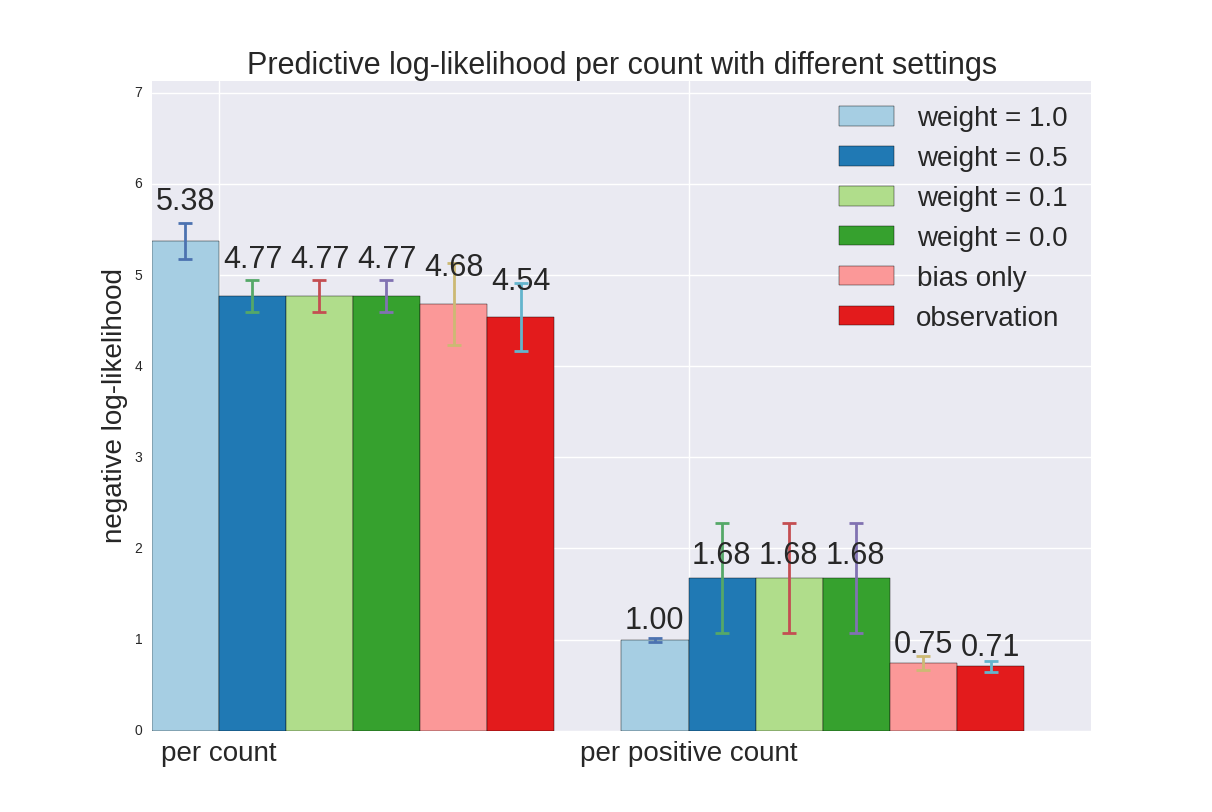
\includegraphics[width=0.6\textwidth]{figures/dwz.png}
    \caption{Negative predicted log-likelihood with different measures of downweighting zeros}
    \label{fig_dwz}
\end{figure}


{\bf Scaling context:} See results in Fig.~\ref{fig_scaling}. It seems that scaling context counts does not help in this task. 
We think some useful signals are destroyed by scaling. 

\begin{figure}[t]
    \centering
    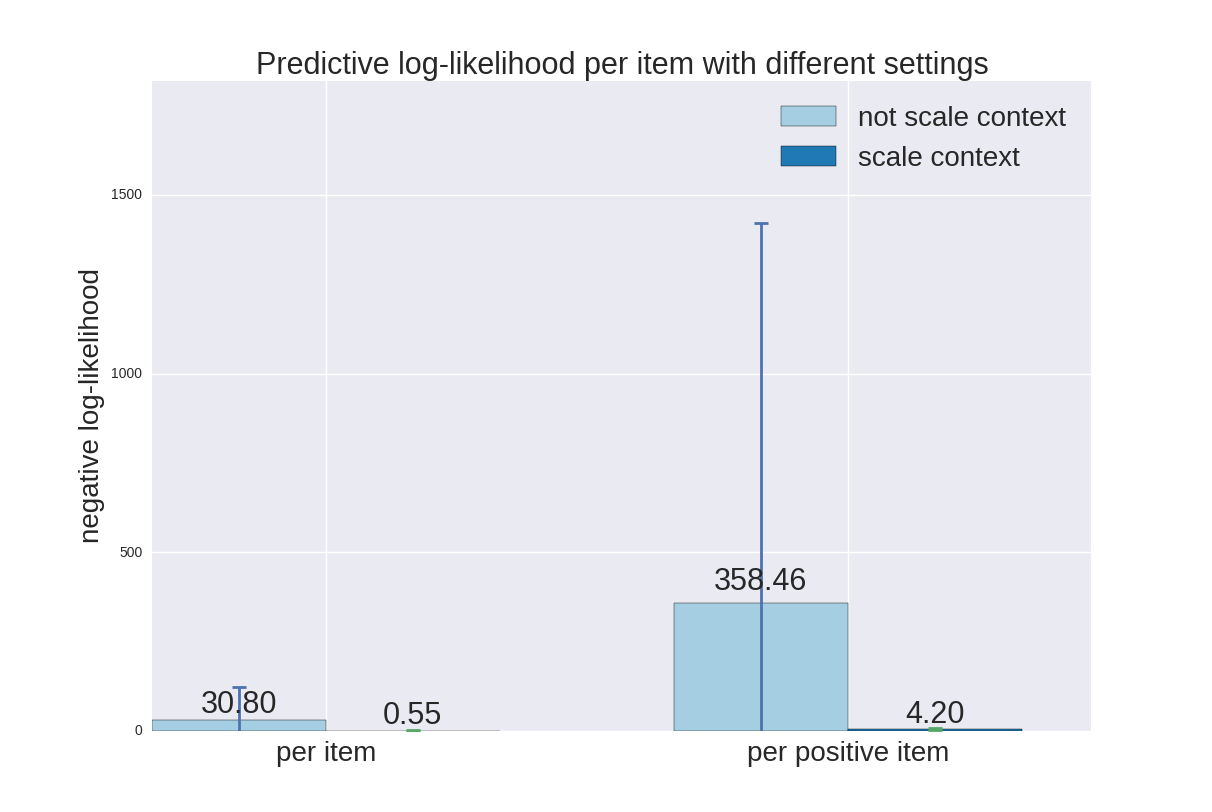
\includegraphics[width=0.6\textwidth]{figures/scale_context.png}
    \caption{Negative predicted log-likelihood with and without scaling the context}
    \label{fig_scaling}
\end{figure}


{\bf Intercept term: } See results in Fig.~\ref{fig_intercept_term}. Intercept terms $\lambda^0$ help to explain the data. 
\begin{figure}[t]
    \centering
    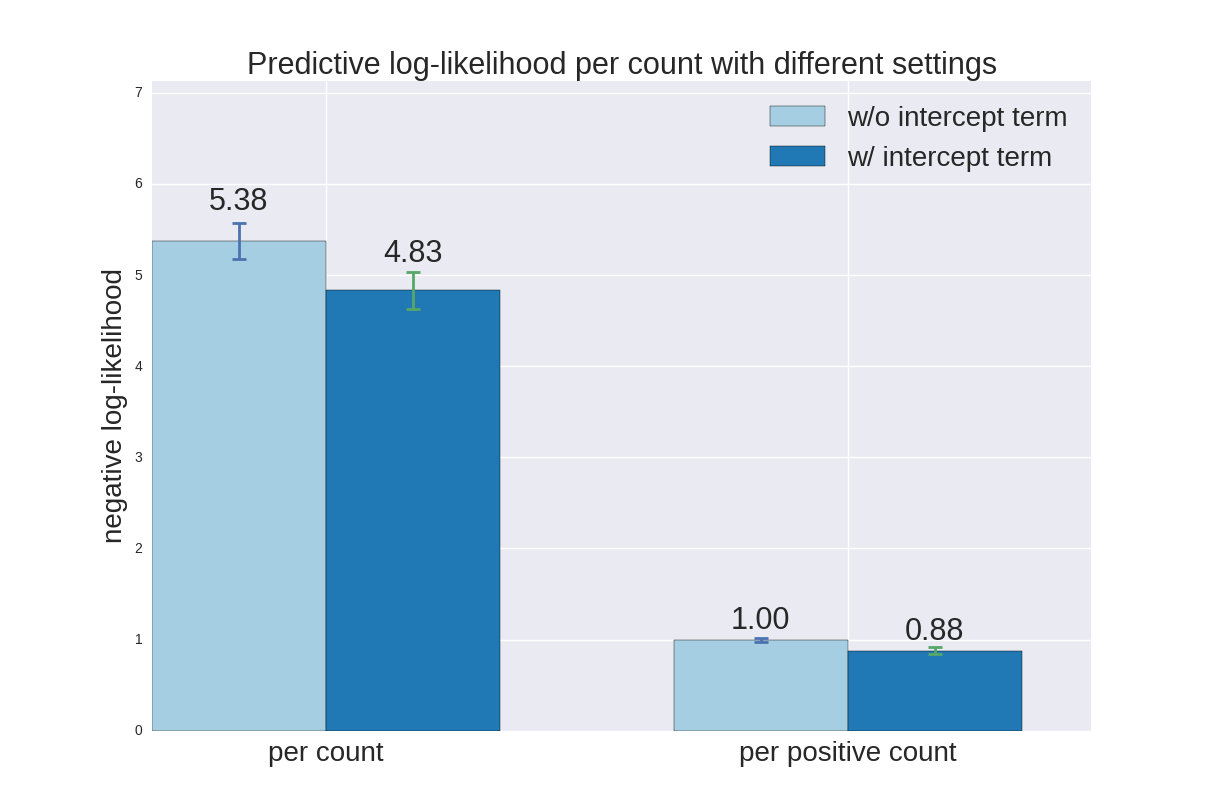
\includegraphics[width=0.6\textwidth]{figures/intercept_term.png}
    \caption{Negative predicted log-likelihood with and without the intercept term}
    \label{fig_intercept_term}
\end{figure}


{\bf Link function:} See results in Fig.~\ref{fig_link_func}. The softplus function gives better results. 
Softplus function is additive while exponential function is multiplicative. 
\begin{figure}[t]
    \centering
    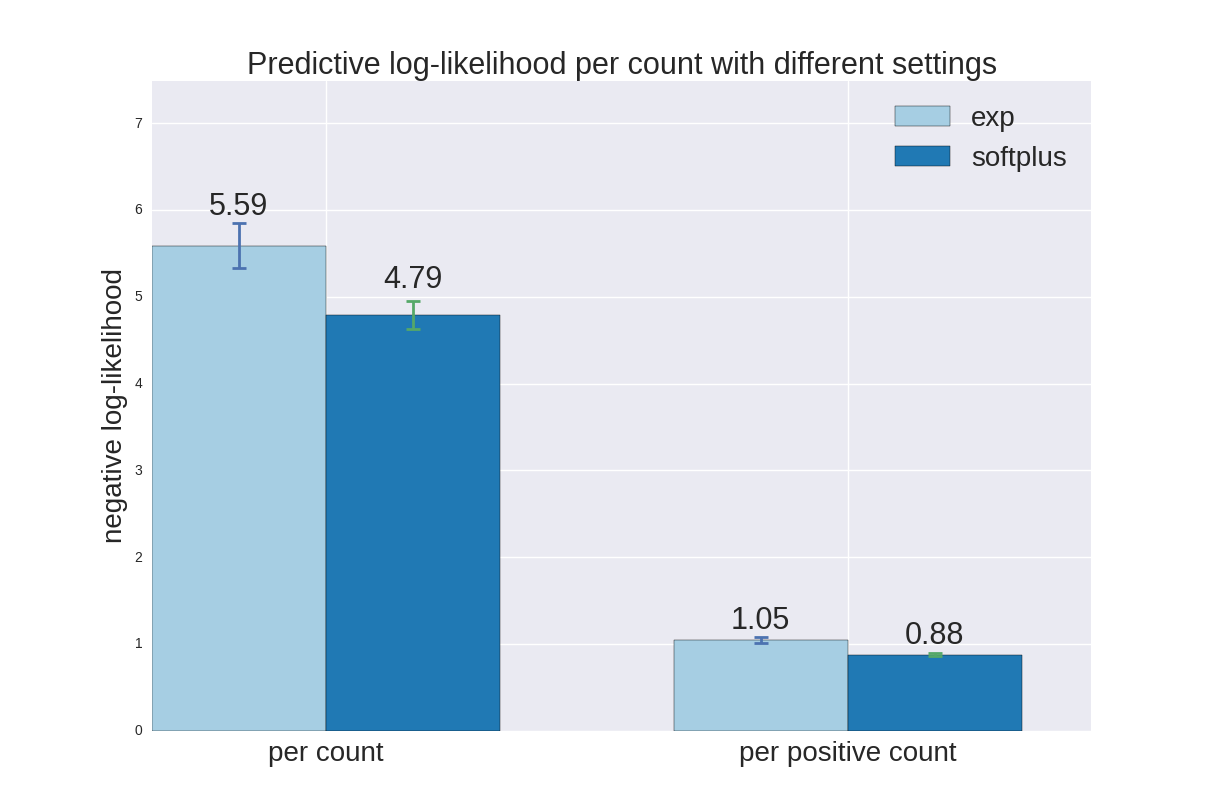
\includegraphics[width=0.6\textwidth]{figures/link_func.png}
    \caption{Negative predicted log-likelihood with $\exp$ and $\mathrm{softplus}$ as the link function}
    \label{fig_link_func}
\end{figure}

{\bf Number of dimensions:} See results in Fig.~\ref{fig_dimensionality}. Larger embedding dimension gives better performance in this range.  
\begin{figure}[t]
    \centering
    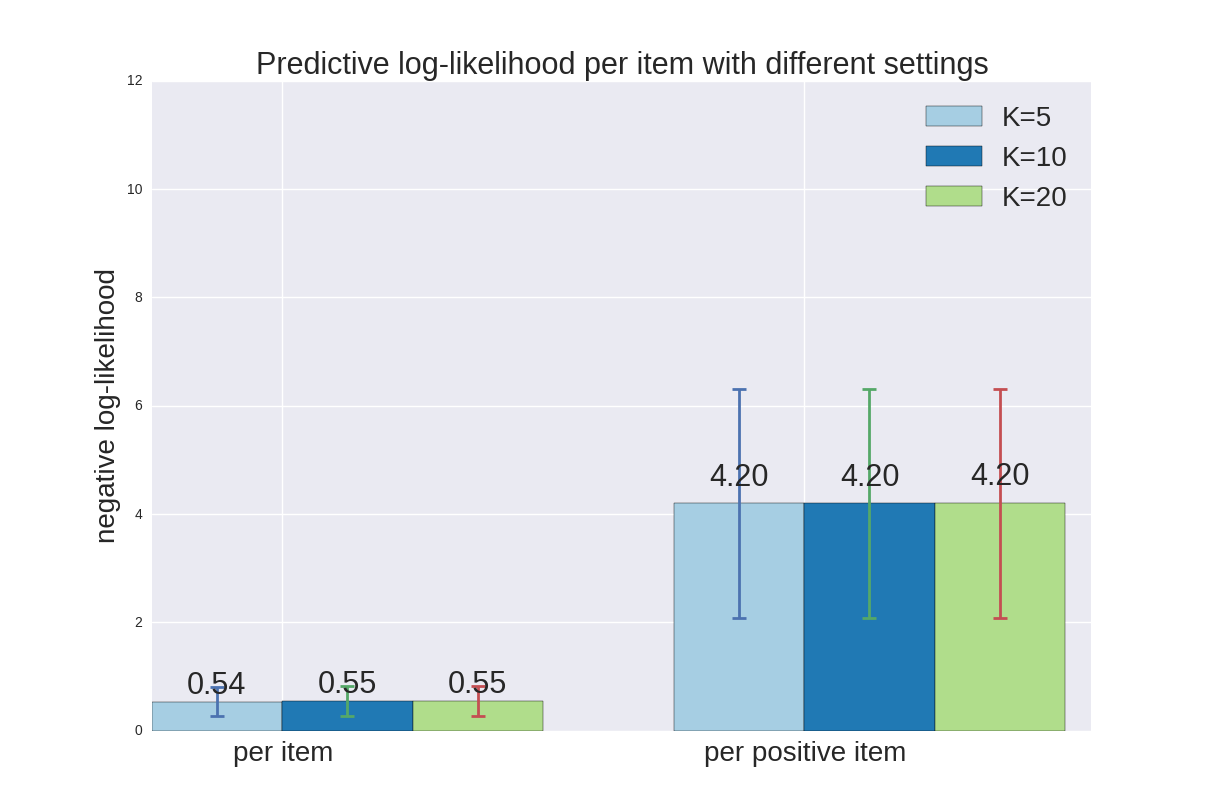
\includegraphics[width=0.6\textwidth]{figures/variate_K.png}
    \caption{Negative predicted log-likelihood with different dimensionalities}
    \label{fig_dimensionality}
\end{figure}

{\bf Embedded vectors:}
We also plot out the embedded vectors of bird species in Fig. (\ref{fig_emb_bird}). 
The model settings are $K = 10, \sigma_1 = \sigma_2 = \sigma_3 = 100, f(\cdot) = \mathrm{softplus}(\cdot)$, and the exposure model is used. 

\begin{figure}[t]
    \centering
    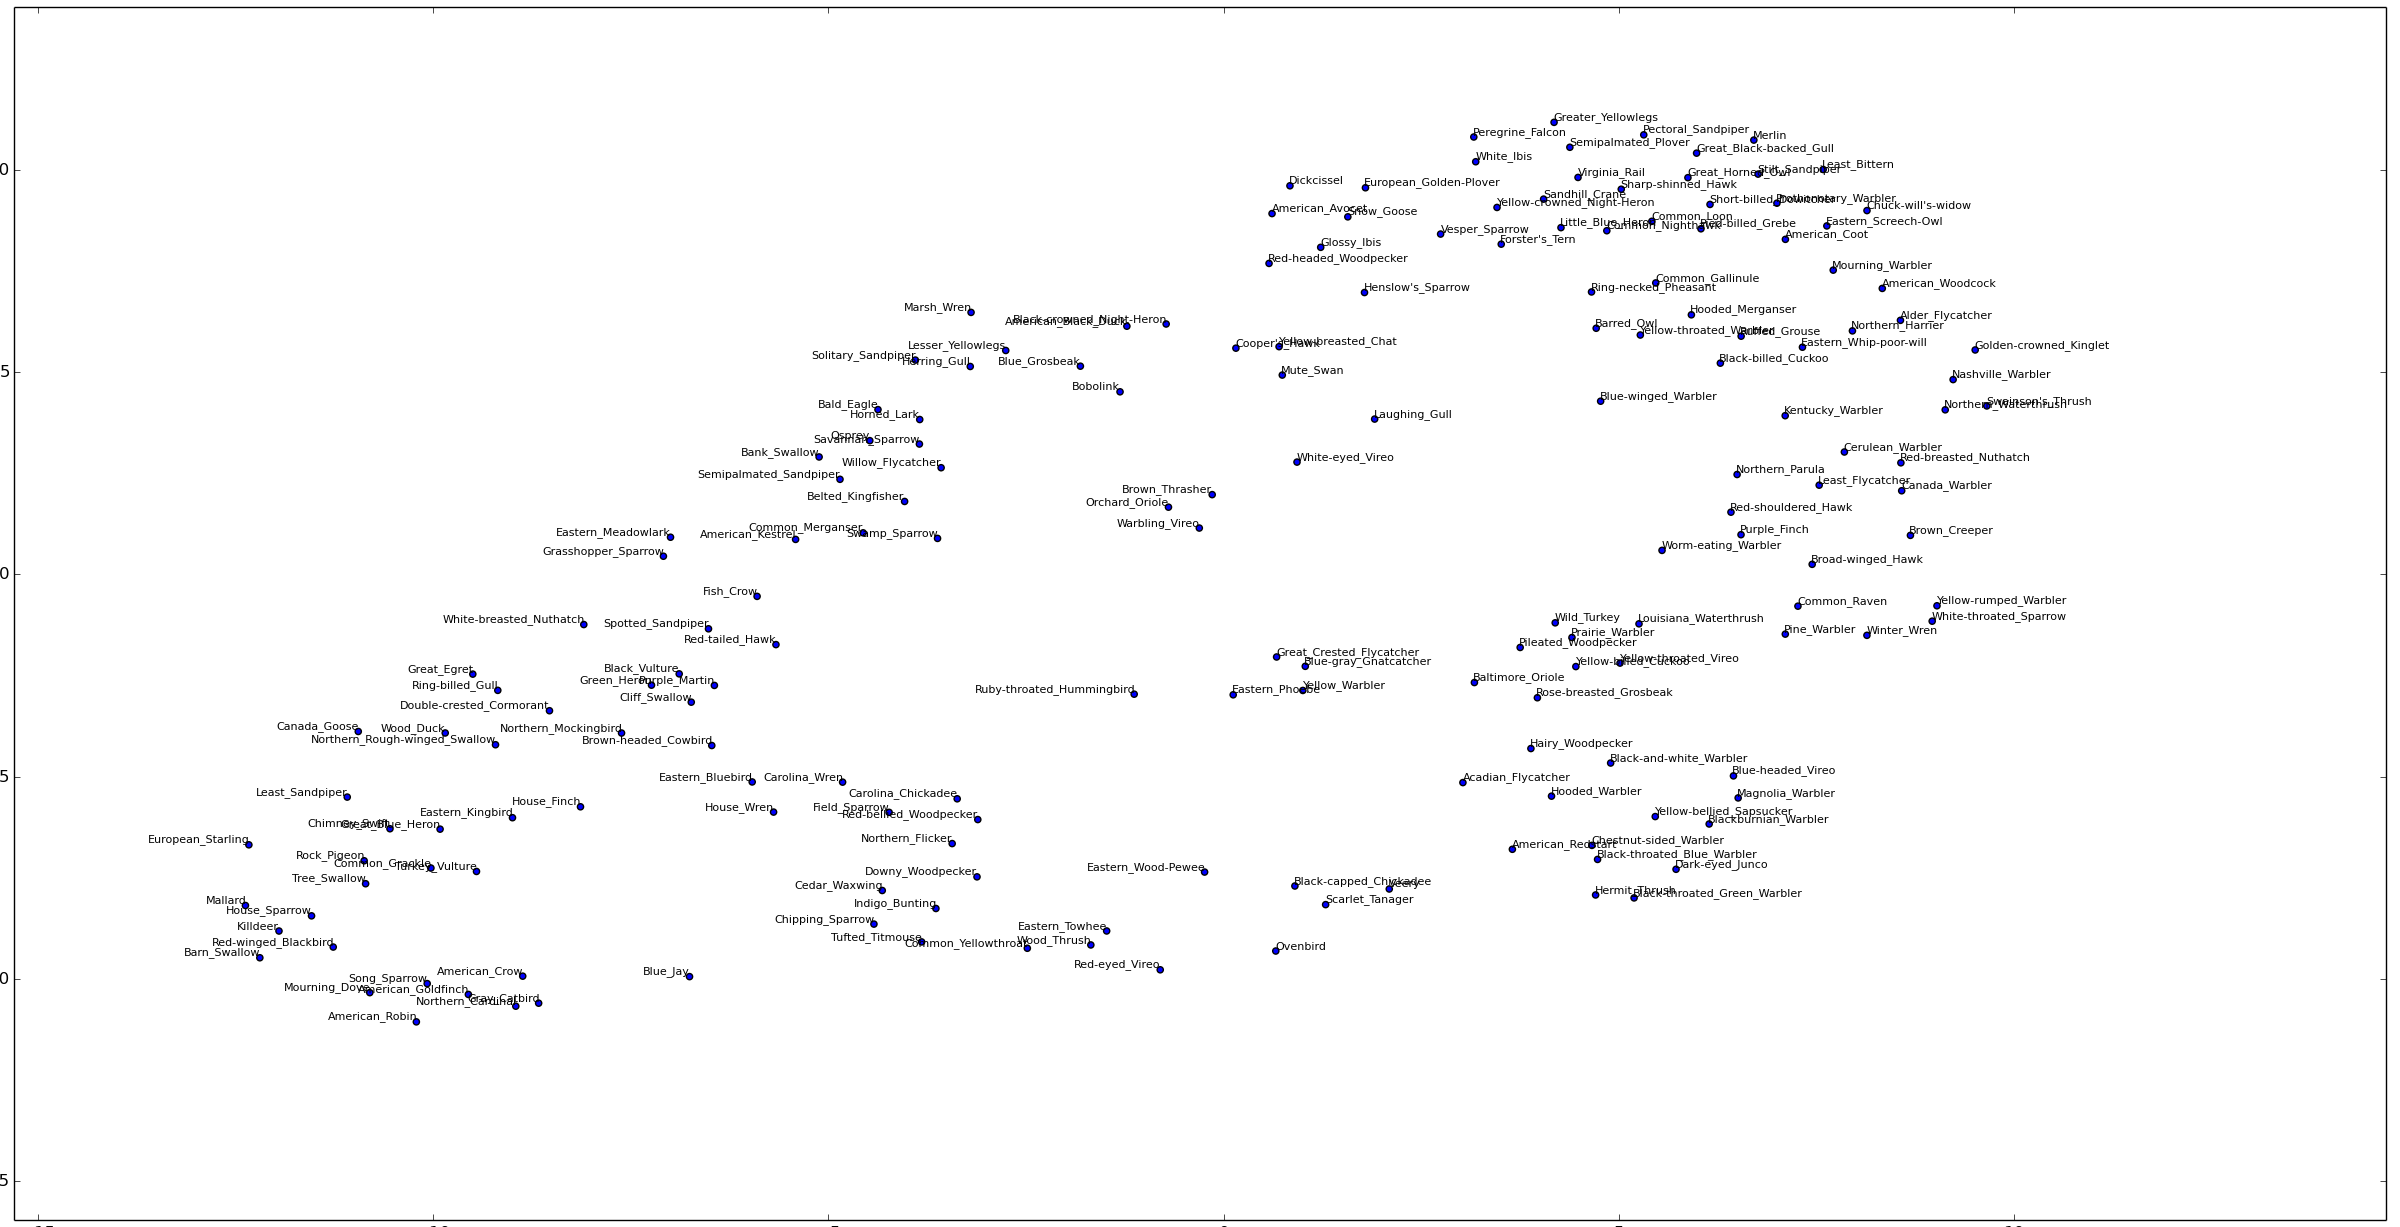
\includegraphics[width=1.0\textwidth]{figures/embedded_birds.png}
    \caption{Embedded vectors for different species}
    \label{fig_emb_bird}
\end{figure}



\section{Research Directions}

Check the effect of parameter initialization. 

Average context of checklists from the same area. 

Use negative binomial distribution instead of Poisson. 

Assumption: embeddings at similar time-locations are similar but different. Can we use a $\wt_{ij}$ for each checklist $i$ and species $j$ and put a GP prior over $\wt_{ij}$-s to encourage strong correlation among $\wt_{ij}$-s at neighboring locations?  

Can we predict the presence/absence of species?

\end{document}

